% !TEX root = DesignDocument.tex

\chapter{Prototypes}

This chapter is a log of the various stages of the DanceSoft prototype. Each prototype is organized by the South Dakota School of Mines Senior Design class sprints.   

\section{Sprint 1 Prototype}

The goal of the first sprint was to collect the requirements for the project. Once requirements gathering was complete the team moved to a research phase with the end goal of deciding on how the three main parts of the project would be implemented. These three parts where the programming language, the user interface framework, and the database type. Through the research the team came to three decisions.

The first of these was the programming language. The team choose Python as this iterations programming language. Python has the upside of being a language the team is more experienced in. Also the client Dr. McGough knows Python so any updates would be easier for him to work on should he decide to work on the project after this team is disbanded. Python is also a cross platform language which allowed the team to produce working code for Mac, Windows, and Linux at the same time. This means the the team can develop on Windows, a development environment we are more familiar with overall. Also development in Python means that if the Academy was ever sold to a Windows user the product would still work. Another advantage we discovered to python is the academic and career experience it provide since in our research for the SD Mines career fair we discovered that many companies use Python and more than expected would like QT experience. Lastly the Python community is larger and can more readily provide assistance if needed through websites and research. This does not mean that other languages like Swift were not viable choice but the time spent learning a completely new language and its GUI toolkit would have added significantly to the project learning curve and reduce even further the amount the team could have completed.

The second part of the research was the GUI toolkit. After looking into GUI kits like Kivy and PyQt the team decided to go with PyQt as Kivy would have added to much to the ramp up time. Also PyQt provide easy to use tools for GUI design through things like the Qt designer, and more help within the community.

The last research was in database type, the database aims to store employees and students and classes information and the size of students less than 4000 and the size of employees less than 10. The structure of data is stable, by considering all those facts above, we decide to use SQL database. For the type of MySQL database, the team thought of using MySQL. MySQL is a free software and widely used in different fields. It has very good portability and can run over different OS systems and aims for small size of data. Also our experience is more focused in MySQL as a part of the South Dakota School of Mines and Technology, and the feature set for SQL in MySQL fits within the scope of the project, for these reasons we choose MySQL as the database frame work.


The last part of the prototype for this sprint was learning the materials we had selected. The team began practice with the PyQt tools and developed a sample window to learn the basic things available for the system.\\

\subsection{Deliverable}
\begin{enumerate}
\item The research into program languages, database and GUI frameworks and architectures for the DanceSoft project.
\item Final decision on frameworks and architectures for the DanceSoft project.
\item User Stories and Product Backlog for the project.
\item Creating a simple Qt window.
\end{enumerate}

\subsection{Backlog}
\begin{enumerate}
\item Set up Github (source control)
\item Design Research
\item Design Decision
\item Create first window
\item Sprint 1 documentation
\item Sprint 1 Review
\item Continuing practice with QT

\end{enumerate}

\subsection{Success/Fail}
The team was able to make framework decisions and begin to learn the toolkits for use in the project. Overall this sprint was a success.\\

\section{Sprint 2 Prototype}
As of now the prototype is in a state to begin working on functionality. The rough (not final) GUI pages are laid out and being constructed to give us an environment for creating the functionality. The back end database has been constructed and will allow us to begin testing the database connected page as we create them. Current pages constructed are log in page, landing pages, and some options pages.

The first thing we tackled in this prototype was getting the database up so we could begin actually developing the product and give our qt interface something to actually interface with. The main goal here was to make sure we had constructed the database in such a way that it could complete all the user stories it needed to in a way that made sense. After talking through the tables and the users stories we came up with the table creation script.

\begin{figure}
\caption{Tables currently in database}
\centering
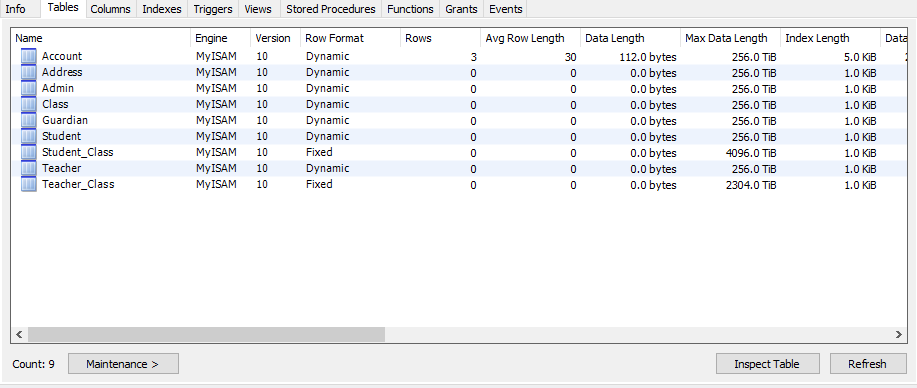
\includegraphics[width=0.5\textwidth]{database_tables}
\end{figure}

The GUI pages for this sprint were the log in page and the landing pages for admin and teachers. The first page the team constructed  was a log in in page that takes a user name and a password and first checks to see if they exist and are correct within the database. If they are not a dialog saying whats wrong appears and prompts the user again. If the information passes the check the system reads the users permission level and sends them to the corresponding landing page.

\begin{figure}
\caption{Current iteration of the log in page}
\centering
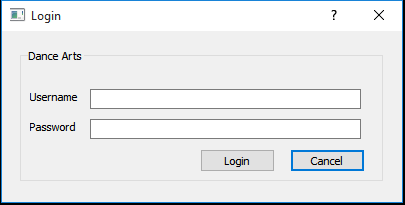
\includegraphics[width=0.5\textwidth]{login_page}
\end{figure}

The other set of pages we need to make to begin writing functionality was the landing pages for the admin and teacher permission levels. These pages show the types of things each can do and allow navigation to the various different functionality. For example the admin landing page has a button to take the user to a student options page, from there the user can select which option they want and will be taken to the page to execute that function.\\


\subsection{Deliverable}

\begin{enumerate}
\item The database creation script  
\item GUI path work
\item Log in page that reads users permission level and sends them to the correct landing page
\item Rough landing pages for Admin and Teachers (design improvements to come in later sprint) 
\end{enumerate}

\subsection{Backlog}

\begin{enumerate}
\item Creation of database tables 
\item Draw GUI path
\item Create a log in page that sends the user to the correct landing page based on their permission level
\item Create versions of teacher and admin landing pages to test functionally (improve look in latter sprint 
\item Continue GUI page creation to have environments for functionality 
\item Sprint 2 Review
\item Continuing practice with QT
\end{enumerate}

\subsection{Success/Fail}
The team was able to produce the log in page and the landing pages for both admins and teachers. The team was also able to create the database on the School of Mines server and get the general structure of the tables up and running. The team did begin to experience issues with time owing to the loaded academic commitment of both team members. Also causing issues was the teams inexperience with PyQt and each other. The team communication was flawed in execution and inexperience on the part of both team members with the GUI caused further slow down.\\


\section{Sprint 3 Prototype}
The progress is being made on the simpler functions of the projects including search, updates, and role sheets. As of now the prototype is in a state of some working functionality on the admin and teacher side. The pages are not yet tied together but the complete functions function independently. Several GUI pages are complete or in a working state to compliment these functions. The back end database has been slightly updated to adjust to the needs of the project. Lastly the prototype has reached a state where testing can be conducted on parts of the project.

The first page tackled was the search page. The page takes user input and searches based on name using a fuzzy search. Also included in both searches is an advanced search option that allows the user to check boxes corresponding to the fields in the database, which in turn allows the user to search in more versatile ways. Lastly the user can click on a student to pull up all of their information and modify it as needed.\\

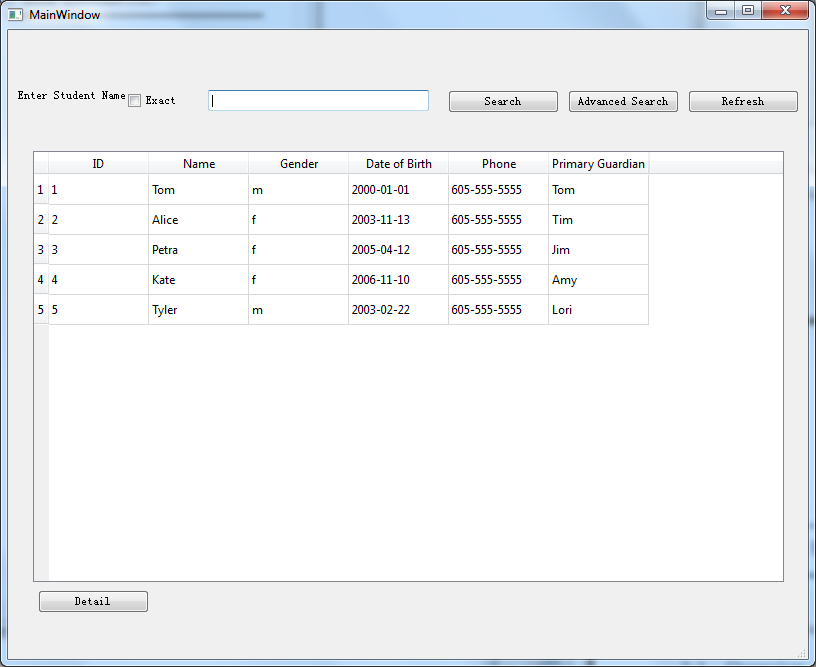
\includegraphics[width=0.5\textwidth]{search.png}

Another page prototype is the "Add a Class" page, by clicking on the "Add a Class" button on the admin landing page will open a dialog. From this dialog box the user can type in information to a add a class to the database. The role sheet page generates a list of classes teachers are currently teaching. Teachers can then see which students are enrolled to take his or her class by selecting the corresponding class on the list. If the user wants they can print this list as a pdf.

Further pages added during this sprint were the update pages. These pages are fairly simple to explain, sometimes the users of the system will need to add or alter a record of some kind these pages need to be able to do so in a simple and concise way. The update pages worked on in this sprint include student information from the employee side, updating teacher information and updates to clothing requirements for a class. Most of these page will just produce a form where information can be displayed and updated.

The assign teacher to class page allows an admin to select a class, clicking on a class pulls up a list of available teachers to select to teach the class. Clicking on a teacher will pull up a message box to confirm the selections before submitting to the database. The available teachers are selected based on the start time of the selected class and the end time of the classes already being taught by each teacher. If the selected class is already assigned the user is prompted with a dialog where the user can select whether or not they would like to reassign the class to a different teacher.\\



\subsection{Deliverable}

\begin{enumerate}
\item Student search page 
\item Employee search page
\item Add a class to the database
\item Update teacher and student information pages
\item Modify clothing requirements for a class
\item Generate a class role sheet
\item Assign teacher to a class
\item Ability to add and subtract students from a class  
\end{enumerate}

\subsection{Backlog}

\begin{enumerate}
\item Queries in database to retrieve student and employee information
\item Query and insert information needed to create and new class and produce a results page.
\item Query database to produce class role sheet
\item Create clothing requirement update function, and add clothing function for teachers and admin
\item Create update query to assign teachers to a class
\item Create ability for employee to look up and modify student information
\item Add and subtract students from a class
\item Sprint 3 Review
\item Create Client presentation
\end{enumerate}

\subsection{Success/Fail}
The team was able to complete several main pages contents to various user stories. However the weight of other academics slowed the teams progress and of course the with the knowledge of the tools growing it was less of a problem then before but still persisted.\\

\section{Sprint 3.5 and 4 Prototype}
During sprint 3.5 the team organized the functionality and tied them together to create the single current working prototype. Other updates were made to fix known bugs and add a class search function. While the team worked on putting the project together smaller bugs or needed pages that were implied by user stories were tackled as they came up. This resulted in too much time being used, so the student interface was not tackled. The student interface has since been dropped from the clients project requirements due to time.

Sprint 4 was dedicated to payroll and billing. First the client rewrote the user stories to provide more clarity to the team. After this the user stories were tackled by the group to produce the first draft of the payroll and billing interface. This included logging hours, payments, fees, rates, and credits. After this sprint the team demoed the project for the client and got notes on the project as a whole. These notes will be tackled as part of the backlog in the next sprint.\\

Prorated Refunds:
The prorated refunds code will keep track of how much a class costed a student. If the student drops a class it will refund the remaining worth of the class to the students school credit field. This file is still in progress at the time of this prototype.\\

Enter Staff Hours:
This page allows an admin to log teacher hours and add different pay rates such as driving rate to the system. There is a default class rate for all teachers. This is further address in the success/fail section below.\\

Enter Tuition Rates and Fees:
These pages allow the user to look at the current tuition rates and fees. The user can then update existing rates, add new rates, or remove rates that are no longer needed. Tuition rates are logged in the database as flat minute rates. The user can enter new rates in the form of minutes or hours.\\

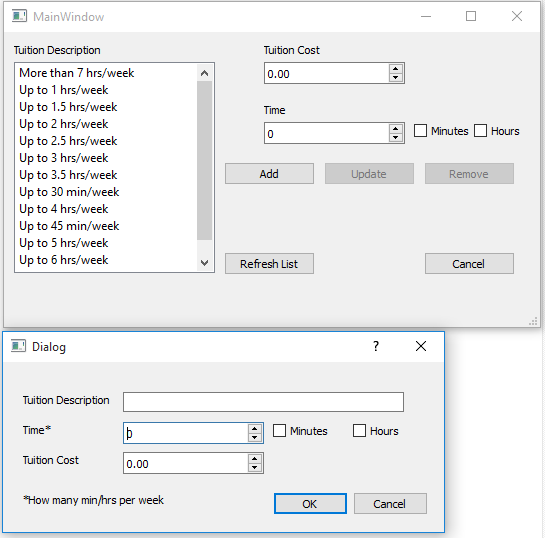
\includegraphics[scale=0.5]{tuitionRates.png}

Teacher History:
This page includes several components. Firstly, user can use this page to find a specific teacher by entering a full or partial name of teachers. Secondly, users can click the history button to open up another window which has a list of classes the teacher has taught.\\

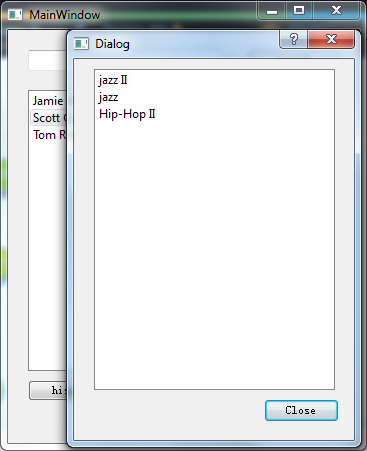
\includegraphics[scale=0.5]{teacherHistory.png}

Set Semester:
This page helps users to set the current semester from pool of semester and add a new semester to the system.

Partial Payment
This page includes several components. Firstly, admin users can use this page to find a specific student by entering a full or partial name of a student into the search bar. Secondly, users can click the pay button to open up another window which asks the user to input amount of money paid, payment methods and semester paid. The user also can choose single or multiple students at one time. \\

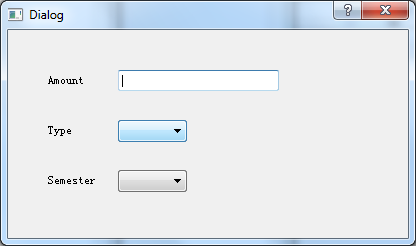
\includegraphics[scale=0.5]{payment.png}

Student's owe:
This page includes several components. Firstly, user can use this page to find a specific student by entering a full or partial name of students. Secondly, users can click the statement button to open up another window which shows the amount of students paid, the amount of students due and the balance of student's account. Users also can print the invoice generated by the window.\\

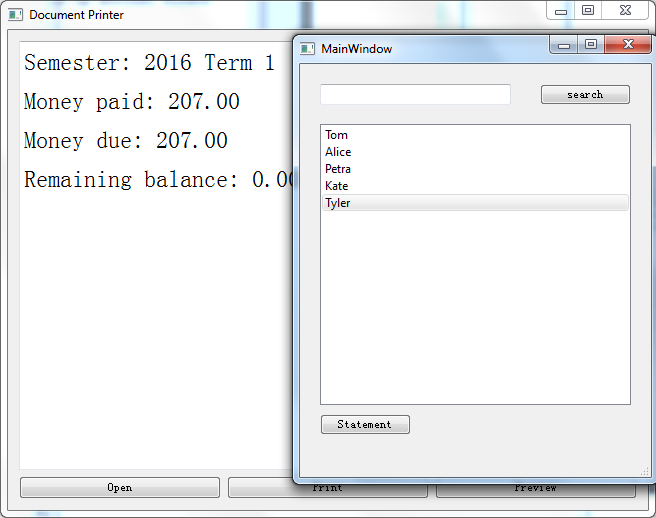
\includegraphics[scale=0.5]{invoice.png}

Enter Payment:
This page includes several components. Firstly, user can use this page to find a specific student by entering a full or partial name of students. Secondly, users can click the clear button to clear the due of selected students. Users can select single or multiple students at one time.\\

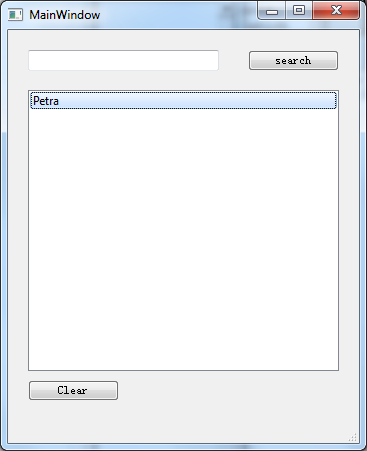
\includegraphics[scale=0.5]{enterPayment.png}

Bill History:
Firstly, user can use this page to find a specific student by entering a full or partial name of students. Secondly, users can click the statement button in order to get the list of payments. In addition, user can print the bill history.\\

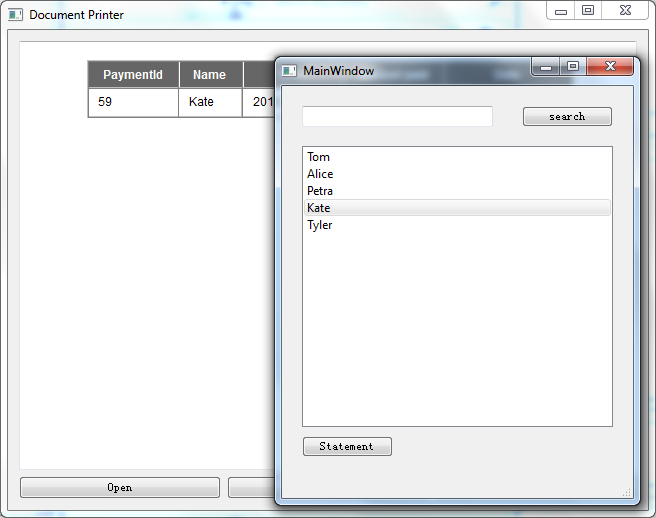
\includegraphics[scale=0.5]{billHistory.png}


\subsection{Deliverable}

Sprint 3.5 had no defined deliverables, and was mostly clean up of user interfaces and functions that were not directly requests by the client but were implied by other client request.

Sprint 4 deliverable was the first draft of the payroll and billing interfaces and functions for the project.\\


\subsection{Backlog}

Sprint 3.5 Backlog:

\begin{enumerate}
\item Fix Assign Teacher to Class Dialog Bug
\item Add Class Search
\item Complete Role Sheet
\item Tie Functions Together
\item Fix Bugs
\end{enumerate}

Sprint 4 Backlog:

\begin{enumerate}
\item View Teaching History
\item Look at The Current Amount Someone Owes
\item Generate an Invoice For The Amount Due
\item Look at Billing History
\item Apply Credits to a Students Account
\item Enter the Tuition and Fees Rate
\item Give Early Registration Discounts
\item Enter Staff Pay Rates
\item Enter a Full Payment for One Student 
\item Enter a Full Payment for Several Students
\item Enter Payments From Multiple Sources For One or More Students
\item Compute Teacher Wages 
\item Enter Staff Hours
\item Give Prorated Refunds 
\end{enumerate}


\subsection{Success/Fail}

During this sprint the team was able to finish most of the rudimentary billing prototypes during these sprints. Most of the prototyping was spent fixing bugs, adding implied functions and making updates.

During this phase the team realized that the project would not reach completion by the end of the project. So the team met with the client to discuss the student interface. After the meeting it was determined that the team could not complete the student interface in time and if it was attempted it would prevent the completion of the local interface as well. As a side affect of this change the team dropped the accept/remove student function was dropped since the function was meant to approve student web registration, then a local student registration function was added to the local GUI to compensate.\\


\section{Sprint 5 Prototype}
Sprint five was dedicated to finishing the last of the functions and clean up of the project. First the client modified  some requirements for the team. After this the user stories remaining from sprint four were tackled by the group to produce the remaining payroll and billing interface. This included logging hours, and payments. After this was done the team started on bug fixes and quality of life updates such as new buttons and removal functions. The team is currently working on finishing up the student registration. If progress continues at this rate the prototype should be completed functionally for our teams iteration however without some work the prototype may not reach some of the teams desired standards.\\

During sprint five the team tackled the remaining functionally, bugs, and quality updates in an attempt to finish the base project. Removal functions to clean out the database were added, and some client requested quality of life updates were added for this project version. Bugs and glitches were patched up in many functions. Another job of this sprint was to finish the rollover from sprint four since some payroll functions still needed work. Lastly the team tackled student registration since the student interface was dropped from the project requirements in sprint 4. The registration is still in progress at this time, as the team failed to complete this functionality in time for the end of the sprint. However it was completed during final sprint.\\

Prorated Refunds:
The prorated refunds code will keep track of how much a class costed a student. If the student drops a class it will refund the remaining worth of the class to the students school credit field. This file has now been completed but due to client request and Academy no refund policy, the team does not foresee this function being useful to the system since the credits can store this information. However this function in left in the project/proof of concept at the request of the client Dr. Jeff McGough.\\

Enter Staff Hours:
This page needed to undergo changes after meeting with client. The new version will allow a teacher to log their in class hours, office hours, trip hours, etc. These hours will then be paid out at their different rates respectfully. The hours will be logged as single numbers not by days or weeks. This function is now completed, as of sprint 5. However as of sprint 6 this function has been added to the rudimentary billing prototype however the team did not add different course rates for each teacher.\\

Enter Teacher Wages:
This was handled in the database in previous sprints assuming one pay rate. However in talks with the client the academy pays different pay rates based on what part of academy work they are doing. So the page will need to be updated once the list of possible pay rates have been provided by the client. This pages and its updates are still in progress. Like the enter staff hours page the course hour rate is the same among all teachers in this version, this will need to be updated in a future iterations of this project as this team was development frozen before changes could be made. \\

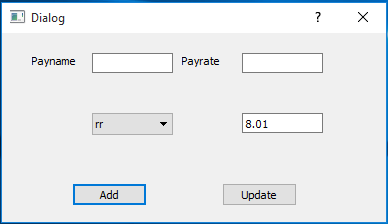
\includegraphics[scale=0.5]{payRates.png}

Enter Tuition Rates and Fees:
Updated these pages to provide quality of life updates to the function requested by the client.\\

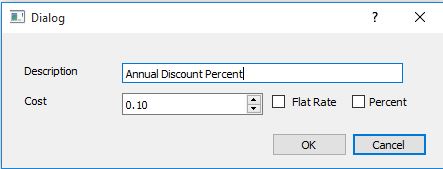
\includegraphics[scale=0.5]{feeDialog.png}

Bug Fixes:
During the course of testing and the client meeting some bugs or inconsistencies were discovered within the project. The bugs found and fixed are:

\begin{enumerate}
\item Student search was not showing all the students. Status: Fixed
\item Search edit need to be turned off and advance search modifications. Status: Fixed
\item Search, role, and schedules need to have dynamic not static times. Status: Fixed
\item Allow for time changes on schedule. Status: Fixed
\item Some of the back buttons in the teacher interface did not work correctly. Status: Fixed 
\end{enumerate}

Updates Crossover:
One of the updates that needed to be completed this sprint was the need for admin and teacher updates to crossover if something was changed. This means that if someone is an admin and they update their phone number through the "update my information form" then the phone number will be updated in both the teacher table and the admin table. This way the system will not have conflicting information in different places. \\

Approved/Rejected Student Updates:
A update requested by the client was the ability to see rejected students in the approved/rejected pages just in case the academy changed its mind about a student. The page underwent slight modifications to the way information was displayed to make this change efficiently. 

Further updates were made in sprint 6, because this function was meant to deal with student approval from the web portal, however since the student interface was dropped from the requirements this function no longer serves a real purpose within the system. If the future when the student portal is added this function may be useful again, as of now the function is left in the project at the request of the client.\\

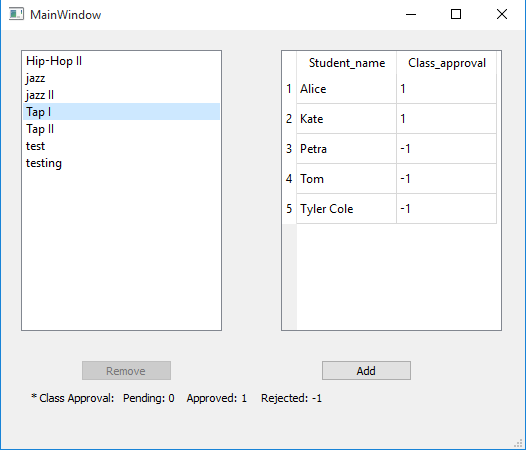
\includegraphics[scale=0.5]{newAddStudent.png}

Admin List:
In creating some of the updates it became clear that a specific admin list was needed to see who had admin access to the system. This was done through a simple list view of the names that can then be selected to display more detailed information about the selected admin.\\


Add/Remove Locations:
Another requested feature was the ability to add and remove locations for classes in the database. This feature is necessary because the Academy sometimes teaches classes in different places based on need. The team accomplished this using a simple dialog that connects to the location field of the class table in the database. When the user updates or adds a new class the location combo box in the form is updated. The user can then select the new location and proceed to finish with class information.\\

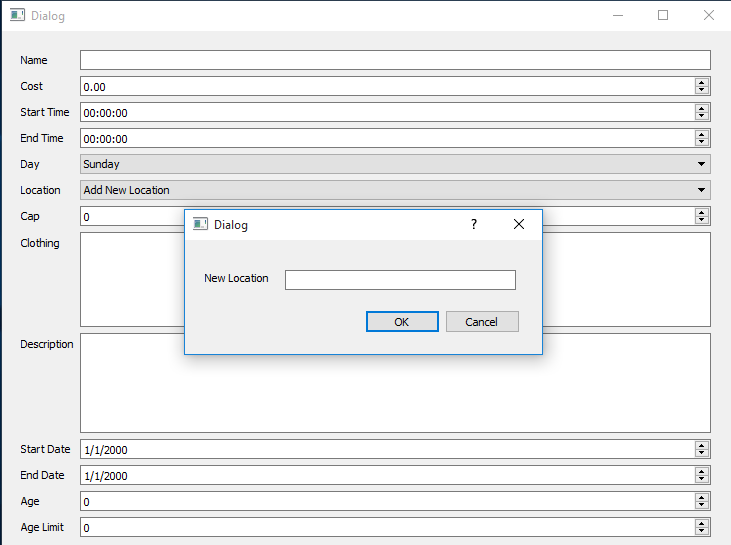
\includegraphics[scale=0.5]{newLocation.png}

Removal Functions:
These are simple functions that pull up a dialog box where the user can select a name and remove all the information related to that user from the system. The removal functions that exist in the system are: teacher, admin, student, and class. Teacher will remove that persons information from the system. Admin removes that persons admin rights and then ask if the whole user should be removed. Student removes all the student information including data, schedules, guardians and addresses. Users should be careful when running any of these functions as the removals are complete and can not be undone or recovered.\\

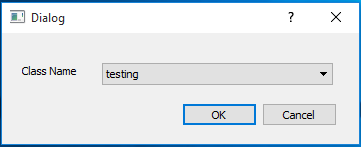
\includegraphics[scale=0.5]{removal.png}

\subsection{Deliverable}

Sprint 5 deliverables were the remaining functionality for the redefined requirements from the client for the project. If the sprint was successful the main project will be done or very close to done functionally for this iteration at the end of the sprint.\\

\subsection{Backlog}

\begin{enumerate}
\item Admin and teacher update crossover
\item Ignoring case in address forms
\item Add rejected students to approved/ reject and provide current status
\item Multiple pay rates
\item Admin list function
\item Enter staff hours
\item Sprint 4 rollover (remaining payroll functions)
\item Add and remove class location
\item Removal Functions (Admin, Class, Student, Teacher)
\item Refunds and check boxes for fees and tuition
\item Quality of life updates to some functions
\item Bug Fixes
\item Student registration
\item Employee wages
\item Begin User Guide for documentation
\end{enumerate}


\subsection{Success/Fail}
At the end of this sprint the project development has been frozen by the client. The project was updated and put together in preparation for South Dakota School of Mines Design fair. As of this final prototype the system has provided the proof on concept now requested by the client. The team will now hand over what was completed to the client along with this document, and the client will decide what to do with the prototype from there.

Since the team was unable to produce a fully functioning project, the project was redefined as a proof of concept for the system and the future of the project will be decided by the client at a later juncture. Since the senior design class has ended and the current DanceSoft team is separating to moving to other projects and jobs.
